\section{Introduction}
The human brain has been a subject of extensive research by the medical image community with a wide range of objectives, from practical clinical applications like disease diagnosis and surgical planning, to addressing scientific questions related to its structure and functionality. The goal of brain image registration is to compute a transformation that brings images of the brain into anatomical correspondence so that they can be jointly analyzed. A rough classification of volumetric image registration methods may be based on two main criteria: a) the deformation model (linear/non-linear), and b) the similarity measure (mono-modal/multi-modal). Registration of images from different modalities (\emph{multi-modal} image registration) is a specially challenging task, since an appropriate similarity metric is harder to define in the multi-modal case than in the \emph{mono-modal} case. Multi-modal image registration has traditionally been constrained to linear methods: since registration of medical images of different modalities is almost exclusively applied to intra-subject image registration, it is often believed that there must exist a linear transformation that correctly brings them into correspondence. However, certain imaging modalities present severe distortions that cannot be accommodated by a linear model. Diffusion MR images, for instance, suffer from distortions caused by $B_{0}$ susceptibility and eddy-currents \citep{Tournier2011, Andersson2003}, which makes their registration to other modality images, even from the same subject, a non-linear problem if these artifacts are not corrected beforehand. Despite the complexity of the task, multi-modal image registration has a wide range of potential applications. Combining diffusion data with T1 MRI, for instance, has the potential of significantly improving tractography \citep{Smith2012, Girard2014}.

\subsection{Multi-modal registration using information theoretic measures}
Existing multi-modal registration methods may be classified into two main approaches: 1) those that optimize information theoretic measures from the estimated joint probability distribution, 2) those that reduce the multi-modal problem to the mono-modal case. The most prominent example of metrics based in information theory is mutual information (MI) \citep{Maes1997, Mattes2003}. The success of MI is explained by its generality, since it does not assume the existence of a functional relationship between the intensities in the two modalities. This generality comes at the expense of disregarding any notion of proximity of intensity values: two intensities will be considered similar only if their estimated joint probability is high, no matter how close they are numerically, which may cause a large number of local maxima \citep[see][Fig. 2]{Roche1998}. In the standard formulation of MI, the joint probability distribution is estimated from the whole image ({\it i.e.}, it is a {\it global} metric), which makes the metric more robust to the effects of noise \citep{Mattes2003}. An important limitation of this kind of global metrics is precisely that the metric depends solely on the (globally) estimated probability distribution, which cannot capture non-stationary relationships between the image intensities \citep{Hermosillo2004}. Since the probability distributions relate point-wise intensity values (intensities of individual voxels), the metric is also insensitive to local image features that are important in non-linear registration like edges and texture \citep{Heinrich2012}. As pointed out by \cite{Sotiras2013}, any random spatial permutation of corresponding pixels would result in exactly the same distribution. A direct approach to tackle the problem of non-stationary intensity dependencies is to use locally estimated probability functions. \cite{Hermosillo2004}, for instance, uses Gaussian kernels centered at each voxel as weighting functions to reduce the contribution of far voxels to the local distribution. A limitation of using Gaussian kernels is the computational cost, as pointed out by \cite{Hermosillo2004}, which makes it necessary to perform some simplifications and use parallel computing. Besides, as we reduce the number of local samples, the estimation becomes more sensitive to noise~\citep{Mattes2003}.

\subsection{Multi-modal registration by reduction to the mono-modal case}
Reducing the multi-modal problem to the mono-modal case may be accomplished by assuming the existence of a {\it transfer function} between the two modalities (a function that maps intensity values of one modality to corresponding intensities in the other). \cite{Roche2000} showed that, assuming the existence of a transfer function, a maximum-likelihood formulation of the registration problem is equivalent to maximization of the correlation ratio (CR). The main drawback of CR is precisely that it relies on the strong assumption of a functional dependency between the two modalities, which in general is not satisfied. However, experimental results have shown that this assumption is not critical for typical brain image registration tasks~\citep{Roche1998}. Being a global metric, CR shares the robustness to noise of MI but also the inability to capture non-stationary relationships between image intensities. However, one of the advantages of CR over MI is that it is sensitive to proximity of intensity values, which may help to reduce the number of local maxima \citep{Roche1998}. An additional advantage is that the CR metric can be computed efficiently from statistics from the images' iso-sets instead of explicitly estimating the joint distribution. Recently, \cite{Arce-santana2014} proposed a similar formulation of the registration problem which also uses the functional dependency assumption. In their work, the transfer function is modeled as a set of hidden random variables whose values can be estimated using the Expectation Maximization (EM) algorithm. Since the assumptions are similar to those made by \cite{Roche1998, Roche2000}, the resulting optimal transfer functions are the same. However, the resulting metric (which is also obtained by maximum-likelihood estimation) differs in that it introduces a measure of uncertainty in the estimated transfer function for each intensity value. This uncertainty appears in the metric as a weighting function that controls the contribution of each voxel intensity, and it helps to alleviate the effect of non-functional and non-stationary dependencies between the two modalities. One of the limitations of the original formulation proposed by \cite{Arce-santana2014} is that it is asymmetric (a limitation shared with the CR metric) in the sense that the transfer function to be estimated must be chosen beforehand (notice that there are in fact two transfer functions mapping intensities from one modality to the other), which may result in very different solutions. Another limitation is that \cite{Arce-santana2014} use an elastic deformation model \citep{Bajcsy1982, Gee1999}, and their optimization strategy consists in a Gauss-Newton iterative algorithm \citep{GVK502988711} that requires to solve a series of large systems of linear equations.

\subsection{Quantitative evaluation}
Besides developing deformation models and metrics, validation is one of the most challenging aspects in image registration. The most accepted validation methodologies, in the mono-modal case, consist in measuring the overlap of manually annotated anatomical regions \citep{Klein2009, Klein2010, Rohlfing2012}. These methodologies have made possible to quantitatively evaluate non-linear registration algorithms and compare their performance in a meaningful way. The Symmetric Normalization (SyN) algorithm developed by Avants {\it et al.}, and made available as part of the Advanced Normalization Tools (ANTS), has been extensively tested in large comparative studies using the aforementioned methodologies and has consistently been reported as one of the most accurate. For multi-modal images, the MI metric is implemented in ANTS, and can be used with SyN for diffeomorphic registration. However, to the best of our knowledge, there are no equivalent studies that quantitatively evaluate the accuracy of non-linear registration algorithms in the multi-modal case, and performance is assessed, in practice, only visually. The reason why validation becomes more challenging in the multi-modal case is that, as far as we know, there are no manually annotated multi-modal image sets publicly available.

\subsection{Summary of contributions}
In this work, we propose an extension to the EM framework proposed by \cite{Arce-santana2014} in a symmetric fashion to simultaneously consider both transfer functions between image modalities. In addition, we minimize the resulting metric in the space of diffeomorphic transformations by using the symmetric diffeomorphic registration framework developed by \cite{Avants2008, Avants2011}. Our optimization strategy is based on Vercauteren's analysis of the \textit{diffeomorphic demons} algorithm \citep{Vercauteren2009} that may be regarded as a Generalized EM algorithm (GEM) \citep{Neal1998}, in which the energy is not fully optimized at each step with respect to the transformations but only reduced at each iteration. As a natural extension, we propose a new metric, called expected cross-correlation, which extends the cross-correlation metric for multi-modal images by taking advantage of the (globally) estimated transfer functions, which makes the estimation robust to noise, while at the same time achieving sensitivity to local features, captured by the cross-correlation computed over local windows. For quantitative evaluation, we propose a validation methodology for multi-modal brain MRI registration methods based on generating semi-synthetic images using real, manually annotated, mono-modal brain images and a synthetic multi-modal template.\\

In summary, our contributions are three-fold: 1) we extended the expectation maximization (EM) framework proposed by \cite{Arce-santana2014} in a symmetric fashion and minimize the resulting metric in the space of diffeomorphic transformations 2) we propose a new metric, called expected cross-correlation, which extends the cross-correlation metric for multi-modal images, and 3) we propose a quantitative validation methodology for multi-modal brain MRI registration methods.

\subsection{T1-B0 registration}

\begin{figure}[t!]
\centering
    \subfloat[]{\label{fig:T1B0_task_example_b0_up}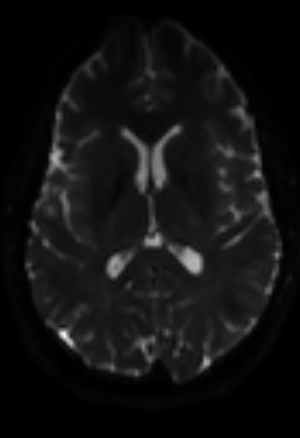
\includegraphics[width=0.3\linewidth]{./images/T1B0Result/T1B0_task_example_b0_up.png}}
    \subfloat[]{\label{fig:T1B0_task_example_b0_down}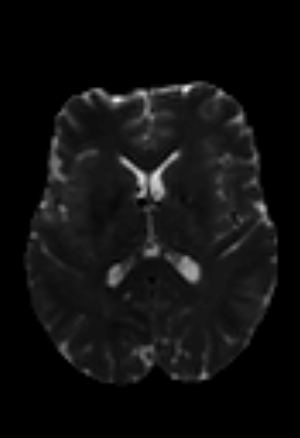
\includegraphics[width=0.3\linewidth]{./images/T1B0Result/T1B0_task_example_b0_down.png}}
    \subfloat[]{\label{fig:T1B0_task_example_t1}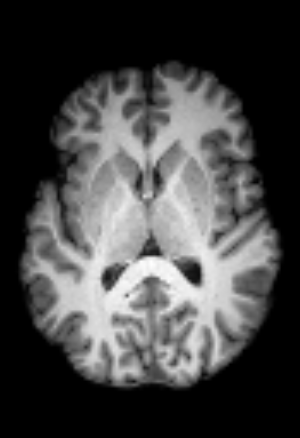
\includegraphics[width=0.3\linewidth]{./images/T1B0Result/T1B0_task_example_t1.png}}
    \caption{Example T1-B0 images from the same subject.}
\label{fig:example_t1b0_problem}
\end{figure}

\begin{figure}[t!]
    \subfloat[]{\label{fig:epicor_b0up_ecc.png}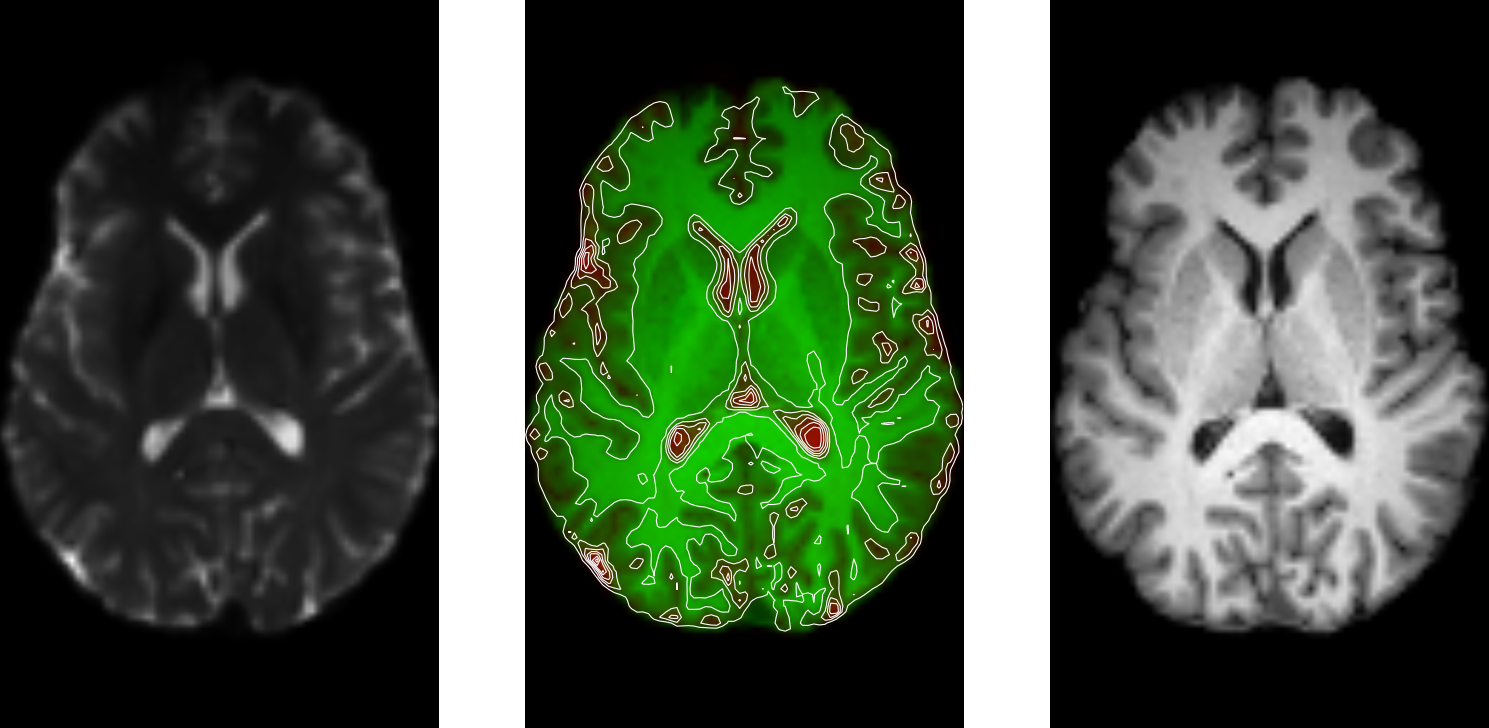
\includegraphics[width=1\linewidth]{./images/T1B0Result/epicor_b0up_ecc.png}}\\
    \subfloat[]{\label{fig:epicor_b0up_mi.png}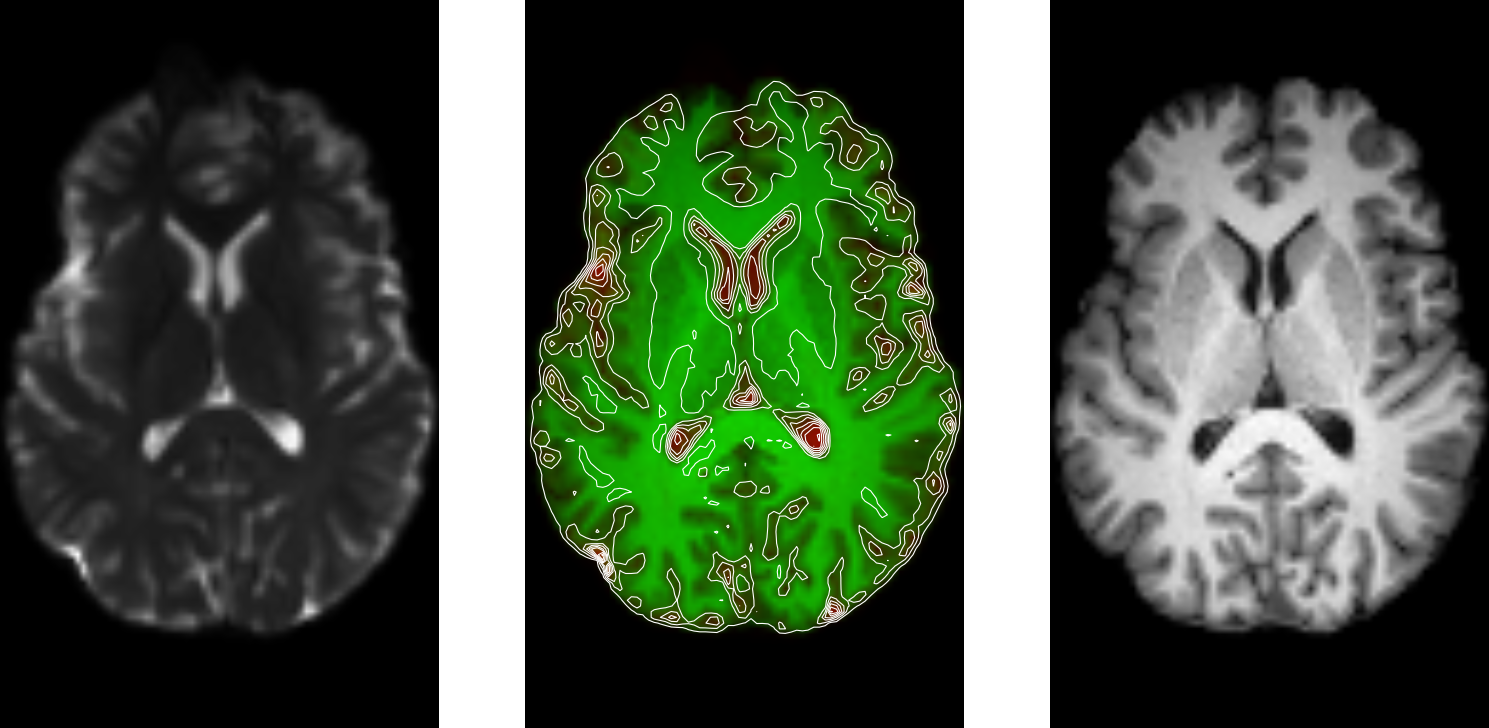
\includegraphics[width=1\linewidth]{./images/T1B0Result/epicor_b0up_mi.png}}\\
    \caption{Registration of B0(blip up) to T1.}
\label{fig:epicor_up_ecc}
\end{figure}

\begin{figure}[t!]
\centering
    \subfloat[]{\label{fig:b0_up_sagital_zoom}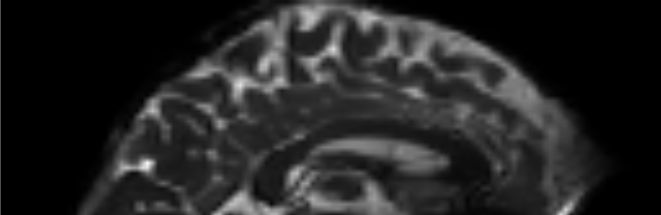
\includegraphics[width=0.5\linewidth]{./images/T1B0Result/b0_up_sagital_zoom.png}}
    \subfloat[]{\label{fig:affine_mi_t1b0up_sagital_zoom.png}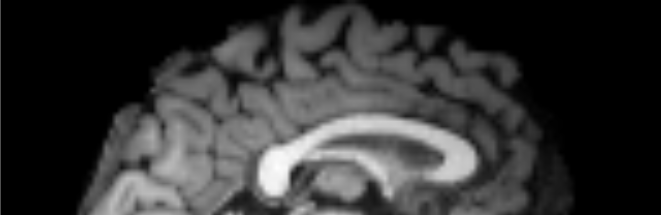
\includegraphics[width=0.5\linewidth]{./images/T1B0Result/affine_mi_t1b0up_sagital_zoom.png}}\\
    \subfloat[]{\label{fig:synecc_contours_t1b0up_sagital_zoom}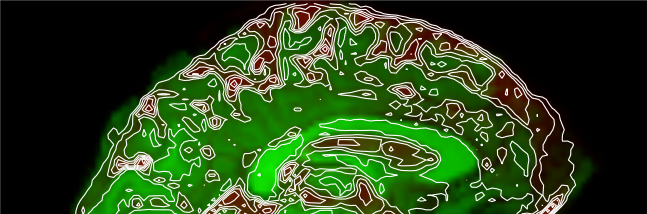
\includegraphics[width=0.5\linewidth]{./images/T1B0Result/synecc_contours_t1b0up_sagital_zoom.png}}
    \subfloat[]{\label{fig:synmi_contours_t1b0up_sagital_zoom}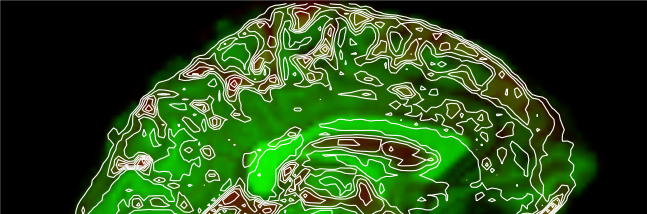
\includegraphics[width=0.5\linewidth]{./images/T1B0Result/synmi_contours_t1b0up_sagital_zoom.png}}\\
    \subfloat[]{\label{fig:synecc_t1b0up_sagital_zoom}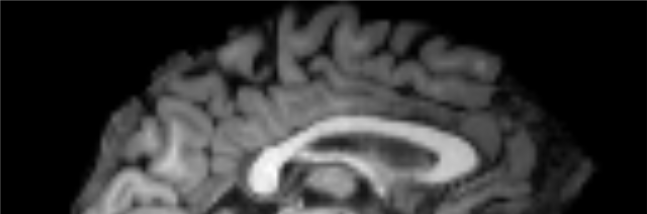
\includegraphics[width=0.5\linewidth]{./images/T1B0Result/synecc_t1b0up_sagital_zoom.png}}
    \subfloat[]{\label{fig:synmi_t1b0up_sagital_zoom}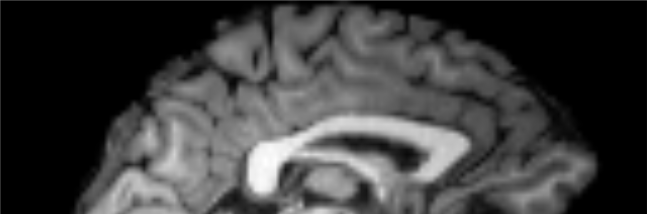
\includegraphics[width=0.5\linewidth]{./images/T1B0Result/synmi_t1b0up_sagital_zoom.png}}\\
    \caption{Registration of T1 to B0(blip up).}
\label{fig:sagital_zoom_t1b0up}
\end{figure}


\begin{figure}[t!]
    \subfloat[]{\label{fig:epicor_b0down_ecc.png}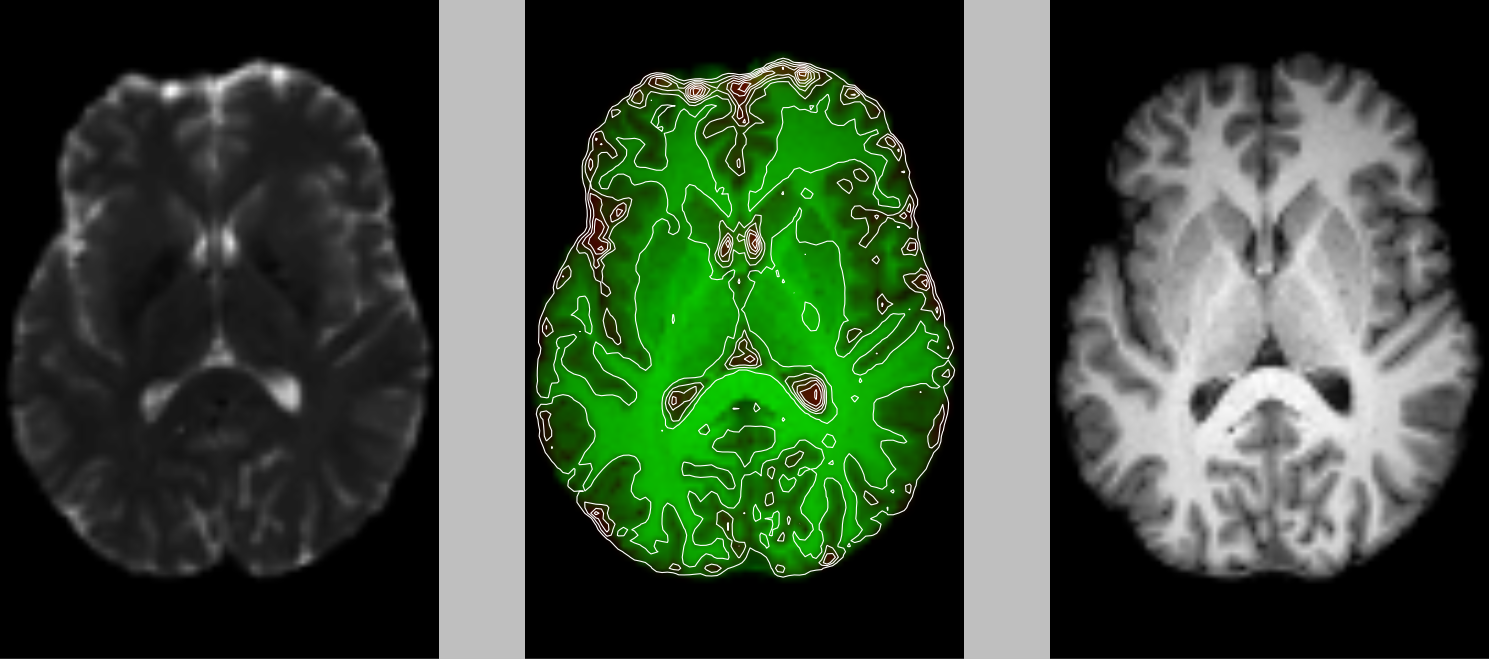
\includegraphics[width=1\linewidth]{./images/T1B0Result/epicor_b0down_ecc.png}}\\
    \subfloat[]{\label{fig:epicor_b0down_mi.png}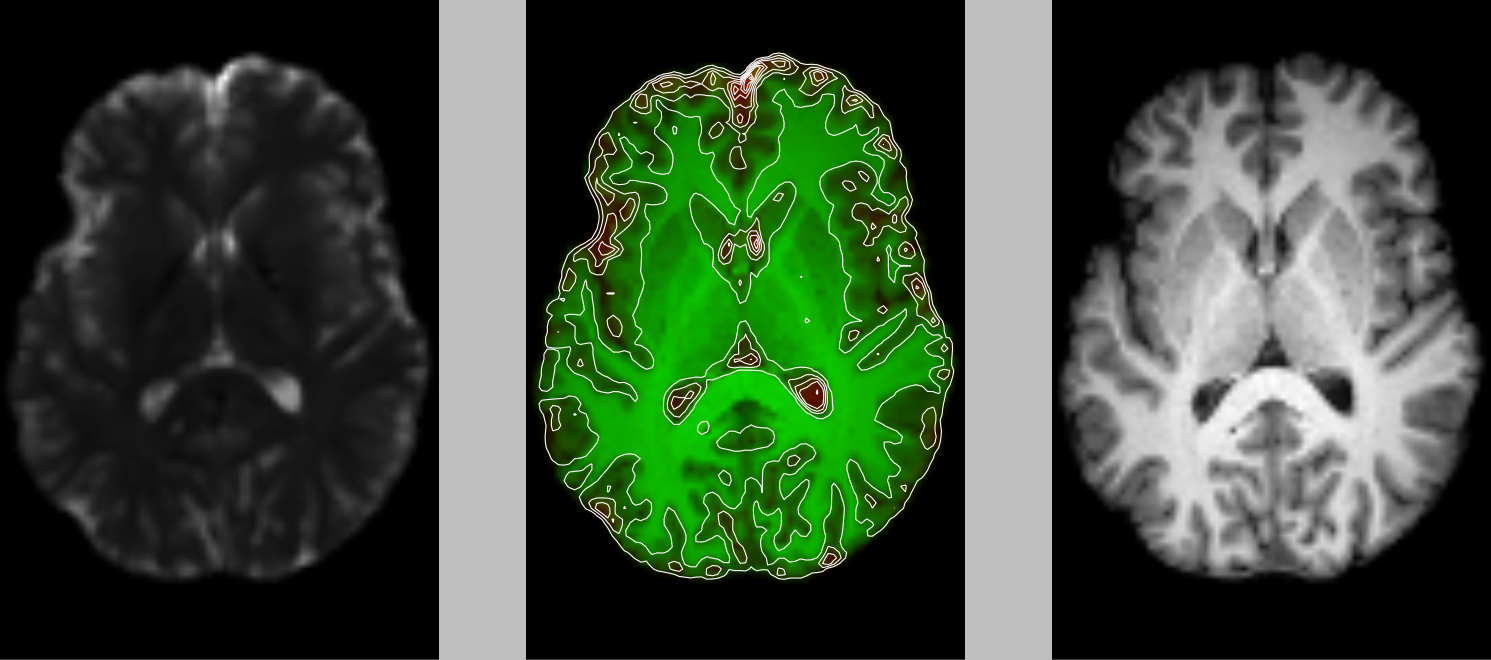
\includegraphics[width=1\linewidth]{./images/T1B0Result/epicor_b0down_mi.png}}\\
    \caption{Registration of B0(blip up) to T1.}
\label{fig:epicor_down_ecc}
\end{figure}

\begin{figure}[t!]
\centering
    \subfloat[]{\label{fig:b0_down_sagital_zoom}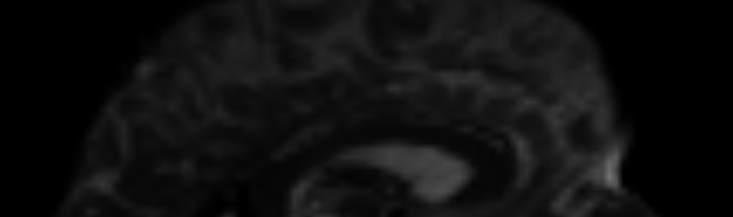
\includegraphics[width=0.5\linewidth]{./images/T1B0Result/b0_down_sagital_zoom.png}}
    \subfloat[]{\label{fig:t1_sagital_zoom}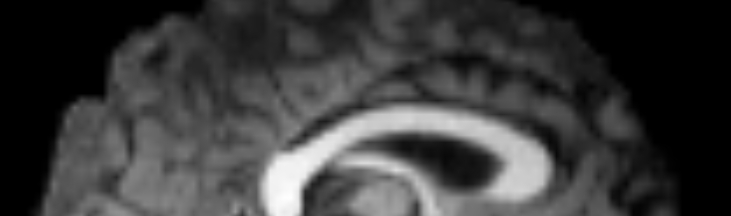
\includegraphics[width=0.5\linewidth]{./images/T1B0Result/t1_sagital_zoom.png}}\\
    \subfloat[]{\label{fig:synecc_contours_t1b0_sagital_zoom}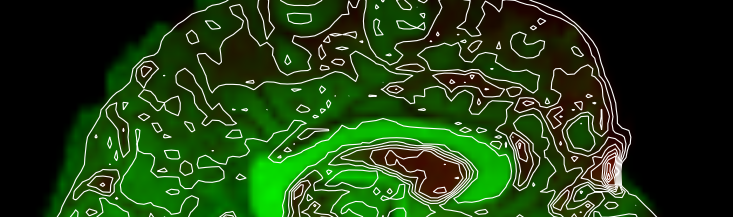
\includegraphics[width=0.5\linewidth]{./images/T1B0Result/synecc_contours_t1b0_sagital_zoom.png}}
    \subfloat[]{\label{fig:synmi_contours_t1b0_sagital_zoom}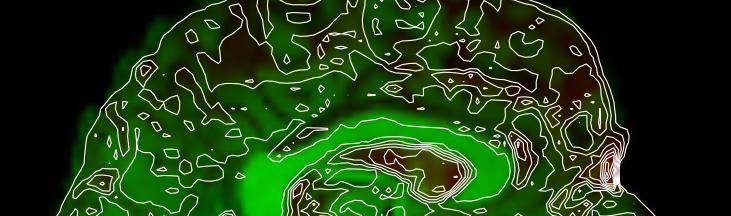
\includegraphics[width=0.5\linewidth]{./images/T1B0Result/synmi_contours_t1b0_sagital_zoom.png}}\\
    \subfloat[]{\label{fig:synecc_t1b0_sagital_zoom}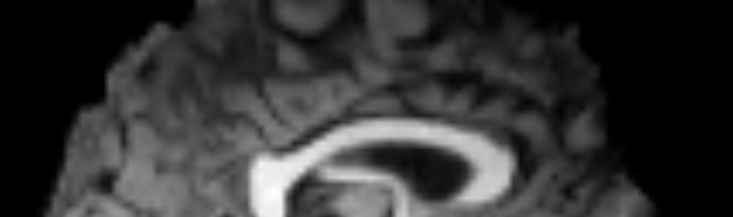
\includegraphics[width=0.5\linewidth]{./images/T1B0Result/synecc_t1b0_sagital_zoom.png}}
    \subfloat[]{\label{fig:synmi_t1b0_sagital_zoom}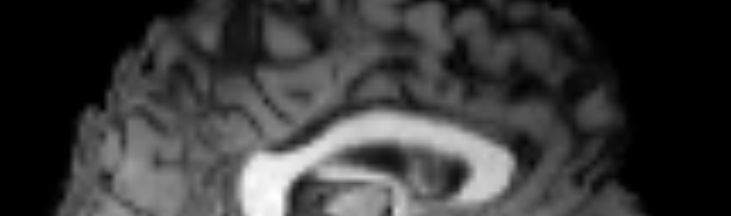
\includegraphics[width=0.5\linewidth]{./images/T1B0Result/synmi_t1b0_sagital_zoom.png}}\\
    \caption{Registration of T1 to B0(blip down).}
\label{fig:sagital_zoom_t1b0down}
\end{figure}


\begin{figure}[t!]
    \subfloat[]{\label{fig:jaccard_T1_B0}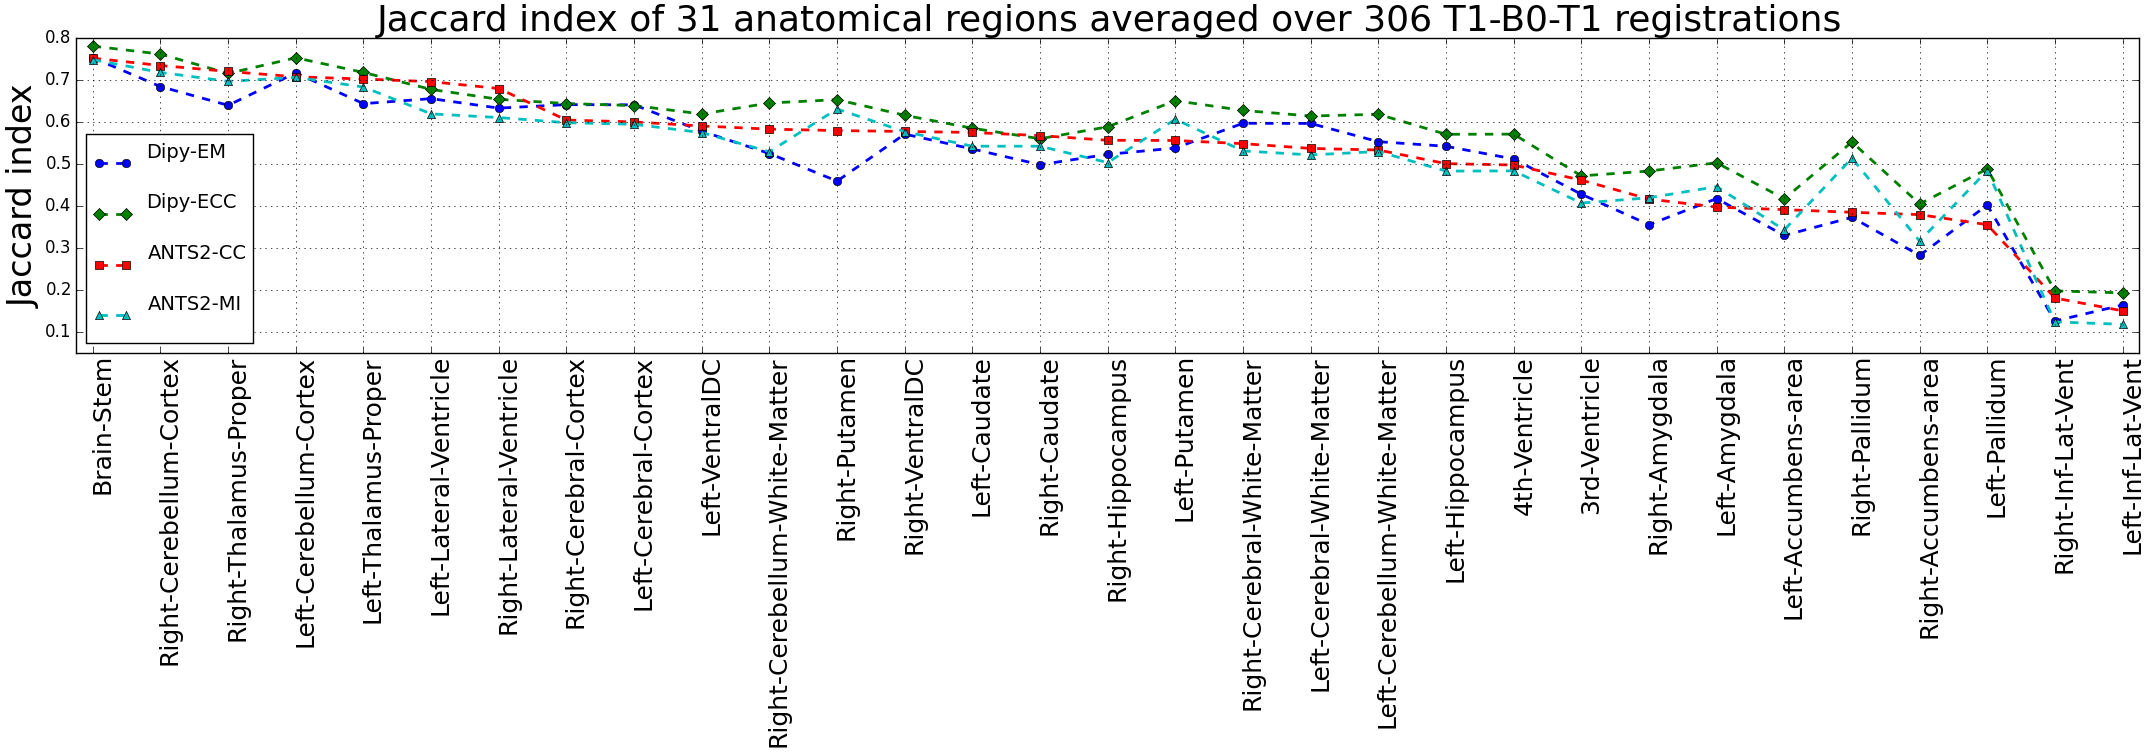
\includegraphics[width=1\linewidth]{./images/T1B0Result/jaccard_T1_B0.png}}\\
    \subfloat[]{\label{fig:jaccard_boxplots_T1_B0}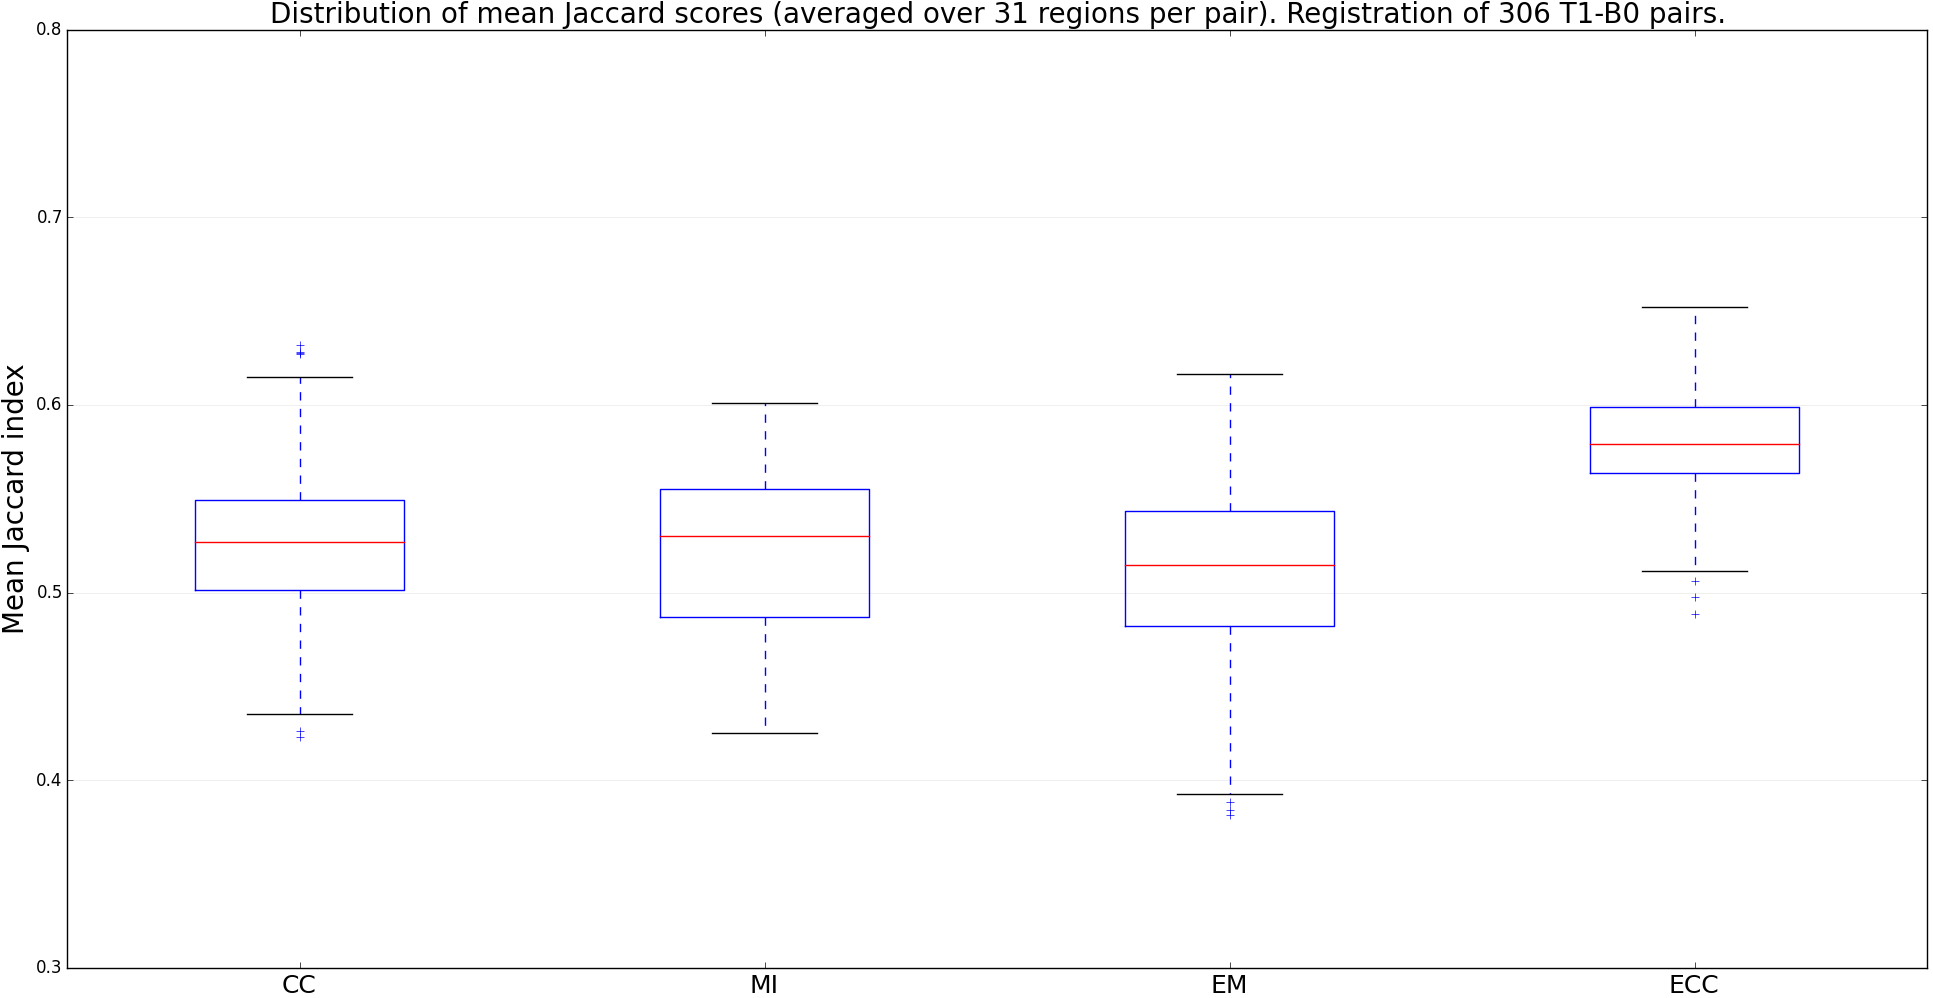
\includegraphics[width=1\linewidth]{./images/T1B0Result/jaccard_boxplots_T1_B0.png}}\\
    \caption{Registration result of B0(blip down) to T1.}
\label{fig:epicor_down_ecc}
\end{figure}


